\normaltrue
\correctionfalse

%\UPSTIidClasse{12} % 11 sup, 12 spé
%\newcommand{\UPSTIidClasse}{11}

\exer{Mouvement T -- $\star$ \label{C2:09:01}}
\setcounter{question}{0}\UPSTIcompetence[2]{C2-09}
\index{Compétence C2-09}
\index{Principe fondamental de la dynamique}
\index{PFD}
\index{Mécanisme à 1 translation}
\ifcorrection
\else
\marginnote{\textbf{Pas de corrigé pour cet exercice.}}
\fi

\ifprof
\else
Soit le mécanisme suivant. On note $\vect{AB}=\lambda(t)\vect{i_0}$. On note $m_1$ la masse du solide \textbf{1}.
On note $G$ le centre d'inertie de \textbf{1} tel que $\vect{BG}=\ell \vect{j_1}$. La pesanteur est telle que $\vect{g}=-g\vect{i_0}$. Un vérin positionné entre \textbf{1} et \textbf{0} permet d'actionner la pièce \textbf{1}. 
On souhaite prendre en compte les frottements secs dans la liaison glissière.
%M et $\inertie{B}{1}=\matinertie{A_1}{B_1}{C_1}{-D_1}{0}{0}{\bas{1}}$.
\begin{center}
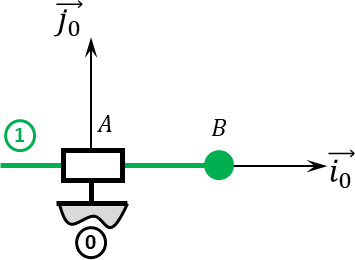
\includegraphics[width=.6\linewidth]{01_T_01}
\end{center}
\fi



\question{Dans le but d'obtenir la loi de mouvement, appliquer le théorème de la résultante dynamique au solide \textbf{1} en projection sur $\vect{i_0}$.}
\ifprof
\else
\fi


\ifprof
\else
\begin{flushright}
\footnotesize{Corrigé  voir \ref{C2:09:01}.}
\end{flushright}%
\fi


